\chapter{Evaluation and Results}

% \section{Introduction}
\section{Evaluation Setup}
  How everything was set up (kubernetes, ml,...)
  
  \subsection{Docker}
  \subsection{Kubernetes}
  \subsection{NetData}

    Netdata is an open source tool that collects real-time metrics, including CPU usage, disk activity, bandwidth usage and further more.
    The reason we chose Netdata for monitoring is that it is a lightweight tool mostly written in C, Python and Javascript and it requires minimal resources, which is necessary when monitoring edge devices.
    One of its major features is that it runs without interrupting any of the applications running on the same device. This is achieved by only using idle CPU cycles while running.

    Netdata provides an in-browser dashboard to analyse each metric in real time with help of visual representation. As an example, a screenshot was taken of a cloud resource in our system as can be seen in \ref{fig:netdata-dashboard}.

    \begin{figure}[h!]
        \centering
        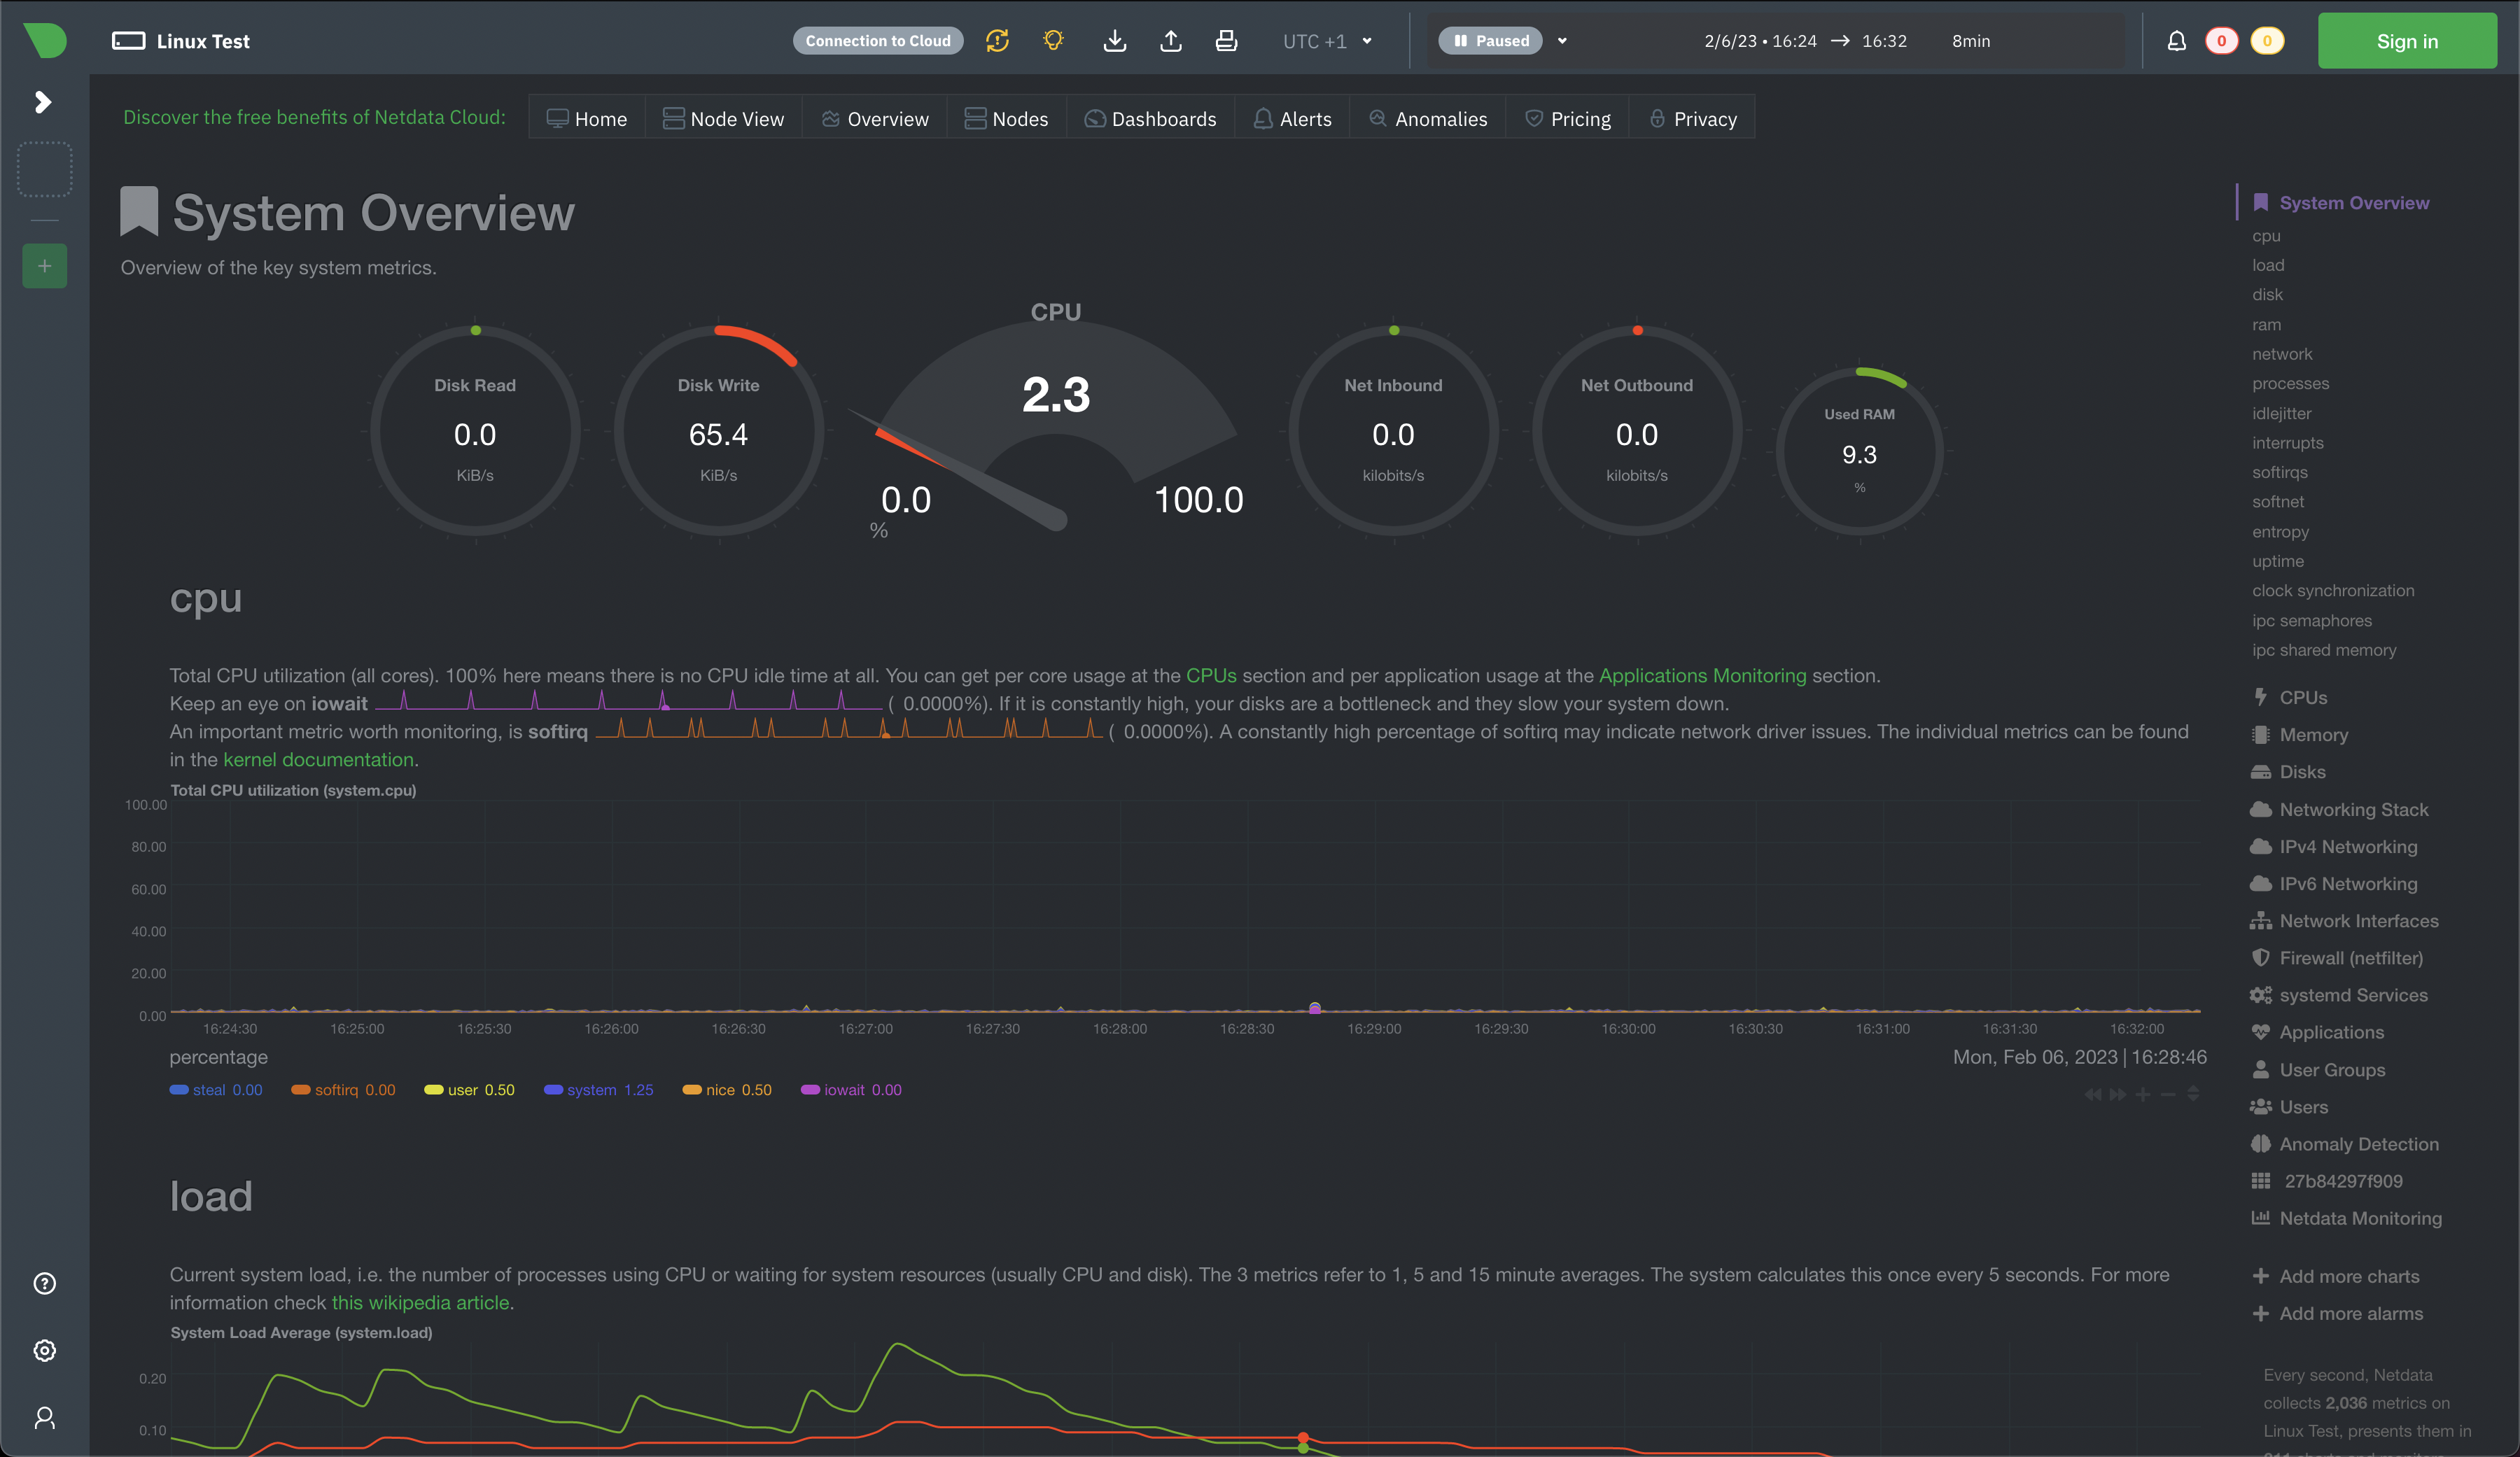
\includegraphics[width=0.95\textwidth]{figures/netdata.png}
        \caption{Netdata Dashboard Example}
        \label{fig:netdata-dashboard}
    \end{figure}
    Netdata has a vast amount of support for other tools in order to gather data. 
    One of the supported tools is \nameref{sec:prometheus-evaluation}, which is used to scrape the monitored data from all resources that have Netdata installed.

  \subsection{Prometheus}
  \label{sec:prometheus-evaluation}
  
    Prometheus is an open source application used for monitoring and alerting of events and is designed to run across various platforms in a scalable and easily deployable manner.
    Same as Netdata it records in real-time, and stores the gathered metrics in a time series database by using a \emph{HTTP pull model}. It also allows real-time alerting via a rule defining configuration and also has a flexible query language called \emph{PromQL}, that enables the retrieval and processing the gathered data. Prometheus has great integration with other tools such as Netdata.
    In the project it is used inside a monitoring master node that is continuously scraping all resources that have Netdata installed for monitoring data. In case a predefined rule is broken at a monitored resource, such as CPU over-allocation, Prometheus triggers an event that notifies ADA-PIPE in order to be able to take measurements.

  \subsection{LSTM Model Setup}
  \subsection{Metrics}

    \paragraph{MAPE}
    \paragraph{sMAPE}
    \paragraph{RMSE}
    \paragraph{Resource Wastage}
      Calculated by subtracting the surface area of allocated - predicted.

  \subsection{Weights \& Biases}
  
\section{Evaluation Scenario}
% the different evaluations I did like task type or batch size
\section{Monitoring}
\section{Data Analysis}
\section{Adaptation}
